\documentclass{beamer}
\usetheme{metropolis}
\usepackage{graphicx}
\usepackage{subfig}
\title{Calculus-Based Physics-1: Mechanics (PHYS150-01): Unit 1}
\date{\today}
\author{Jordan Hanson}
\institute{Whittier College Department of Physics and Astronomy}

\begin{document}
\maketitle

\section{Unit 0 Review}

\begin{frame}{Unit 0 Review}
\begin{enumerate}
\item Methods of approximation
\begin{itemize}
\item \alert{Estimating} the correct order of magnitude
\item \alert{Function} approximation
\item \alert{Unit analysis}
\end{itemize}
\item Coordinates and vectors
\begin{itemize}
\item \alert{Scalars} and \alert{vectors}
\item \alert{Cartesian} (rectangular) coordinates, displacement
\item \alert{Vector} addition, subtraction, and multiplication
\end{itemize}
\item Review of Calculus Techniques
\begin{itemize}
\item Limits
\item Differentiation
\item Integration
\end{itemize}
\end{enumerate}
\end{frame}

\section{Unit 1 Summary}

\begin{frame}{Unit 1 Summary}
\begin{enumerate}
\item Displacement, and instantaneous velocity and acceleration
\begin{itemize}
\item \textit{Mathematics review}: taking derivatives
\item Average velocity and average acceleration
\end{itemize}
\item The case of constant acceleration
\begin{itemize}
\item An \textit{an equation of motion} for constant acceleration
\item Derivation of \alert{common equations of motion}
\item Average quantities and exercises
\end{itemize}
\item \textbf{Lab Activity: Measuring acceleration of gravity: \textit{g}}
\item Exercises with vectors, graphs, and equations of motion
\end{enumerate}
\end{frame}

\section{Displacement, and instantaneous velocity and acceleration}

\begin{frame}{Displacement, and instantaneous velocity and acceleration}
\begin{figure}
\centering
\subfloat[\label{fig:twovectors_a}]{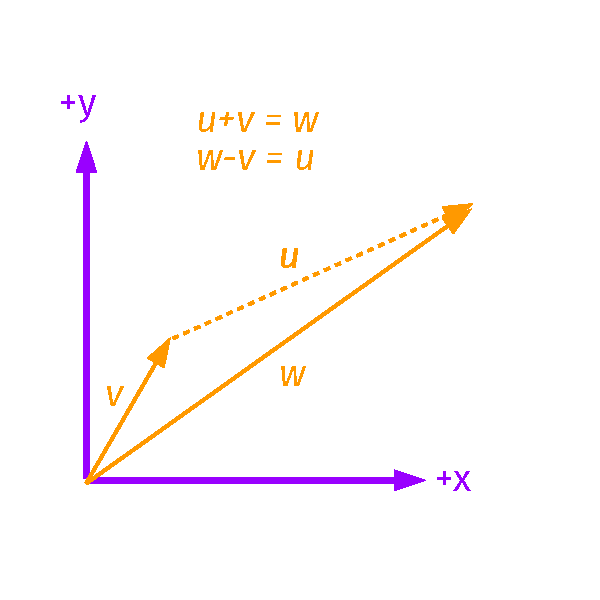
\includegraphics[width=0.45\textwidth]{figures/Vectors4.pdf}}
\subfloat[\label{fig:twovectors_b}]{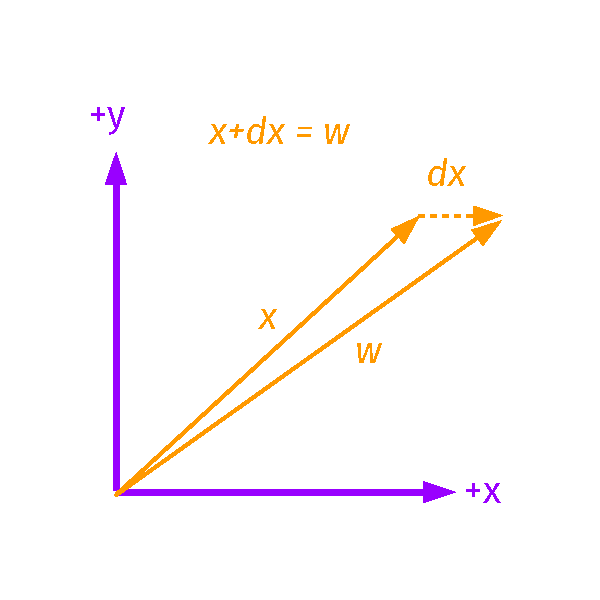
\includegraphics[width=0.45\textwidth]{figures/Vectors1.pdf}}
\caption{\label{fig:displacement} (Left): The displacement vector is $\vec{u}$.  (Right) Treat displacement for a small change in time, $dt$, and call it $d\vec{x}$.}
\end{figure}
\end{frame}

\begin{frame}{Mathematics review: taking derivatives}
\small
\begin{minipage}[b]{0.45\linewidth}
Let $f(t) = A\sin(Bt) + Ct^2$.  \\ Compute $f'$. \\
\vspace{0.2cm}
\begin{itemize}
\item A: $f'(t) = AB\sin(Bt) + 2Ct$
\item B: $f'(t) = AB\cos(Bt) + 2C$
\item C: $f'(t) = AB\sin(Bt) + 2Ct$
\item D: $f'(t) = AB\cos(Bt) + 2Ct$
\end{itemize}
\end{minipage}
\hspace{0.5cm}
\begin{minipage}[b]{0.45\linewidth}
Let $f(t) = (4t-1)/(3t+2)$.  \\ Compute $f'$. \\
\begin{itemize}
\item A: $f'(t) = \frac{4}{3t+2}$
\item B: $f'(t) = \frac{4}{(3t+2)^2}+\frac{12t-3}{(3t+2)^2}$
\item C: $f'(t) = \frac{4}{3t+2}+\frac{12t-3}{(3t+2)^2}$
\item D: $f'(t) = \frac{12t-3}{(3t+2)^2}$
\end{itemize}
\end{minipage}
\end{frame}

\begin{frame}{Displacement, and instantaneous velocity and acceleration}
Definition of instantaneous velocity vector:
\begin{equation}
\boxed{v(t) = \frac{d\vec{x}}{dt}}
\end{equation} \\
\vspace{0.5cm}
Simple example: Let the vector position of an object be
\begin{equation}
\vec{x}(t) = (2t \hat{i} - 3t^2\hat{j}) \quad m
\end{equation}
Then
\begin{equation}
\vec{v}(t) = (2 \hat{i} - 6t\hat{j}) \quad m/s
\end{equation}
\end{frame}

\begin{frame}{Displacement, and instantaneous velocity and acceleration}
Definition of instantaneous \textit{acceleration} vector:
\begin{equation}
\boxed{a(t) = \frac{d\vec{v}}{dt} = \frac{d}{dt} \frac{d\vec{x}}{dt}}
\end{equation} \\
\vspace{0.5cm}
Simple example: Let the vector position of an object be
\begin{equation}
\vec{x}(t) = (2t \hat{i} - 3t^2\hat{j}) \quad m
\end{equation}
Then
\begin{equation}
\vec{v}(t) = (-6\hat{j}) \quad m/s^2
\end{equation}
\end{frame}

\begin{frame}{Displacement, and instantaneous velocity and acceleration}
\textit{Interesting...} If the motion of an object is \textit{quadratic} in time, then the acceleration is a constant. \\
\vspace{0.2cm}
Let the displacement versus time of an object be \\
\begin{equation}
\vec{y}(t) = (-\frac{1}{2}gt^2 + v_{i}t + y_{\rm 0}) \hat{j} \quad (m)
\label{eq:freefall1}
\end{equation}
If Eq. \ref{eq:freefall1} gives the displacement in the $\hat{j}$ direction, then what are the velocity and acceleration?
\end{frame}

\section{The case of constant acceleration}

\begin{frame}{The case of constant acceleration}
Using the definitions of instantaneous velocity and acceleration: \\
\begin{equation}
\frac{d\vec{y}}{dt} = (-gt + v_{i}) \hat{j} \quad (m/s)
\label{eq:freefall2}
\end{equation}
\begin{equation}
\frac{d}{dt}\frac{d\vec{y}}{dt} = (-g) \hat{j} \quad (m/s^2)
\label{eq:freefall3}
\end{equation}
The acceleration is just some constant, $g$, in the $-\hat{j}$ direction.  This leads to a \textit{linear} equation for the velocity, and a \textit{quadratic} equation for the displacement.
\end{frame}

\begin{frame}{The case of constant acceleration}
So we have the following three equations for a system experiencing constant acceleration:
\begin{align}
\vec{y}(t) &= (-\frac{1}{2}gt^2+v_{\rm i}t+y_{\rm 0}) \hat{j} \quad (m) \label{eq:threemain1} \\
\vec{v}(t) &= (-gt + v_{\rm i}) \hat{j} \quad (m/s) \label{eq:threemain2} \\
\vec{a}(t) &= (-g) \hat{j} \quad (m/s^2) \label{eq:threemain3}
\end{align}
What if we solve for time in Eq. \ref{eq:threemain2}, after taking the magnitude of the vector? \\
\begin{equation}
\frac{v-v_{\rm i}}{-g} = t
\label{eq:subt1}
\end{equation}
\end{frame}

\begin{frame}{The case of constant acceleration}
Now substitute Eq. \ref{eq:subt1} into Eq. \ref{eq:threemain1}:\\
\begin{align}
y &= -\frac{1}{2}g\left(\frac{v-v_{\rm i}}{-g}\right)^2+v_{\rm i}\left(\frac{v-v_{\rm i}}{-g}\right)+y_{\rm 0} \label{eq:threemain4} \\ 
-2g(y-y_{\rm 0}) &= (v-v_{\rm i})^2 + 2v_{\rm i}(v-v_{\rm i}) \label{eq:threemain5} \\
-2g(y-y_{\rm 0}) &= v^2-v_{\rm i}^2 \label{eq:threemain6} \\
-2g(y-y_{\rm 0})+v_{\rm i}^2 &= v^2 \label{eq:threemain7}
\end{align}
Equation \ref{eq:threemain7} provides a way to obtain the velocity of an accelerating system at some displacement without knowing the time.
\end{frame}

\begin{frame}{The case of constant acceleration}
A particle moves along the x-axis according to $x(t) = (10t-2t^2)\hat{i}$ m.  What is the instantaneous velocity
at $t=2$ seconds and $t=3$ seconds? What is the average of these two numbers?
\begin{itemize}
\item A: 2 m/s, -2 m/s, 2 m/s
\item B: 2 m/s, 4 m/s, 3 m/s
\item C: 10 m/s, 8 m/s, 9 m/s
\item D: 2 m/s, -2 m/s, 0 m/s
\end{itemize}
\end{frame}

\begin{frame}{The case of constant acceleration}
Let $x(t) = (10t-2t^2)\hat{i}$ m, from prior exercise.  What is the displacement between $t=2$ seconds and $t=3$ seconds?
\begin{itemize}
\item A: 0 m
\item B: 10 m
\item C: -4 m
\item D: 3 m
\end{itemize}
\end{frame}

\begin{frame}{The case of constant acceleration}
Notice in the previous two problems: the \textit{instantaneous velocity} is not the \textit{average velocity}.  The average velocity between two and three seconds was 0 m/s, but the instantaneous velocity was not zero at either point.  However, the \textit{displacement} was 0 m in this time interval.  The \textit{average velocity} must be \\
\begin{equation}
\boxed{\bar{v} = \frac{x_{\rm f} - x_{\rm i}}{t_{\rm f} - t_{\rm i}}} \label{eq:avevel}
\end{equation}
\end{frame}

\begin{frame}{The case of constant acceleration}
\small
On February 15, 2013, a meteor entered Earth’s atmosphere over Chelyabinsk, Russia, and exploded at an altitude of 23.5 km.  Eyewitnesses could feel the intense heat from the fireball, and the blast wave from the explosion blew out windows in buildings. The blast wave took approximately 2 minutes 30 seconds to reach ground level.  What was the average velocity of the blast wave?  Compare this with the speed of sound, which is 343 m/s at sea level.
\begin{itemize}
\item A: 35 m/s (10\% speed of sound)
\item B: 100 m/s (30\% speed of sound)
\item C: 150 m/s (40\% speed of sound)
\item D: 350 m/s (100\% speed of sound)
\end{itemize}
\end{frame}

\begin{frame}{The case of constant acceleration}
Notice that if we take the limit $t_{\rm f} \to t_{\rm i}$, or $\Delta t = t_{\rm f} - t_{\rm i} \to 0$, \\
\begin{align}
\lim_{\Delta t \to 0} \bar{v} &= \lim_{\Delta t \to 0} \frac{x_{\rm f} - x_{\rm i}}{t_{\rm f} - t_{\rm i}} \\
\lim_{\Delta t \to 0} \frac{x_{\rm f} - x_{\rm i}}{\Delta t} &= \frac{dx}{dt} = v(t)
\end{align}
The limit of the average velocity as the time interval approaches zero is the instantaneous velocity.  What about acceleration?
\end{frame}

\begin{frame}{The case of constant acceleration}
A particle moves along the x-axis according to $x(t) = (10t-2t^2)\hat{i}$ m.  What is the instantaneous acceleration
at $t=2$ seconds and $t=3$ seconds? What is the average of these two numbers?
\begin{itemize}
\item A: 2 m/s$^2$, 2 m/s$^2$, 2 m/s$^2$
\item B: -4 m/s, -4 m/s, -4 m/s
\item C: -4 m/s$^2$, -4 m/s$^2$, -4 m/s$^2$
\item D: 0 m/s$^2$, 0 m/s$^2$, 0 m/s$^2$
\end{itemize}
\end{frame}

\begin{frame}{The case of constant acceleration}
Notice that the \textit{average acceleration} and the \textit{instantaneous acceleration} are equal.  This implies that the acceleration is constant.  Similar to the definition of \textit{average velocity}, we have the \textit{average acceleration}:\\
\begin{equation}
\bar{a} = \boxed{\frac{v_{\rm f} - v_{\rm i}}{t_{\rm f} - t_{\rm i}}}
\end{equation}
\end{frame}

\begin{frame}{The case of constant acceleration}
A cheetah can accelerate from rest to a speed of 35.0 m/s in 7.00 s. What is its average acceleration, if it's headed in the $-\hat{i}$ direction?
\begin{itemize}
\item A: -5 m/s$^2$
\item B: 2 m/s$^2$
\item C: 10 m/s$^2$
\item D: 5 m/s$^2$
\end{itemize}
\end{frame}

\section{Lab Activity: Free-fall}

\begin{frame}{The case of constant acceleration}
\small
This is a simple lab exercise to see if we understand the kinematic equations well enough to predict where an object will land.  Let's assume we are rolling a marble off the edge of the lab table at some known initial horizontal speed $v_{x,i}$.  When it leaves the table, it will begin to accelerate:
\begin{equation}
v_y(t) = v_{i,y} - g t
\end{equation}
We know that $v_{i,y} = 0$ m/s.  Thus, we know the velocity as a function of time because we know $v_{x,i}$ will not change and $v_y(t)$ is known. \\ \vspace{0.5cm}
Suppose the height of the table is $h$.  Show that
\begin{equation}
h = -\frac{1}{2}g t^2
\end{equation}
Use this equation to solve for $t$. (Remember that the object has $v_{x,i}$, but acceleration is in the $y$-direction.
\end{frame}

\begin{frame}{The case of constant acceleration}
\small
The result should be
\begin{equation}
t = \sqrt{\frac{2h}{g}}
\end{equation}
\begin{enumerate}
\item Measure $h$ with the ruler, and predict $t$.
\item Drop the marble from the height and confirm the prediction using a stopwatch.
\item If the marble was moving at some constant \textit{horizontal} velocity, $v_{x,i}$, where would it land?
\item Roll the marble next to a ruler that is laid on the table such that you can time it and obtain $v_{x,i}$ as the marble leaves the table.  Make sure the ruler is perpendicular to the edge.  Mark where the marble lands and measure the horizontal distance from the table (call it $\Delta x$).
\end{enumerate}
\end{frame}

\begin{frame}{The case of constant acceleration}
Using $\Delta x = v_{x,i} t$, find the predicted horizontal distance of landing, $\Delta x$.  Does it agree with your measurement?  Why or why not?
\end{frame}

\section{Lab Activity: Measuring acceleration of gravity}

\begin{frame}{Lab Activity: Measuring acceleration of gravity}
\small
\begin{figure}
\centering
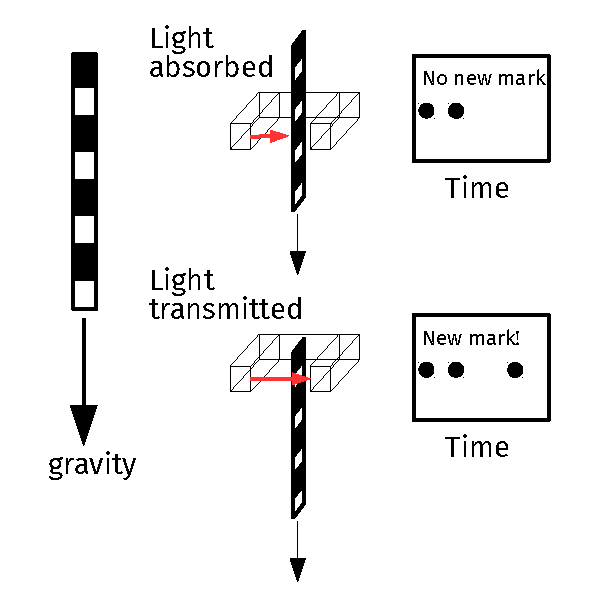
\includegraphics[width=0.5\textwidth]{figures/PicketG.pdf}
\caption{\label{fig:picket} (Left) A \textit{picket} is marked at regular intervals with black strips.  (Right) Upon dropping the picket through a \textit{photo-gate}, the strips will block the photo-gate and we will record when this happens on a clock.}
\end{figure}
\end{frame}

\begin{frame}{Lab Activity: Measuring acceleration of gravity}
\small
\begin{figure}
\centering
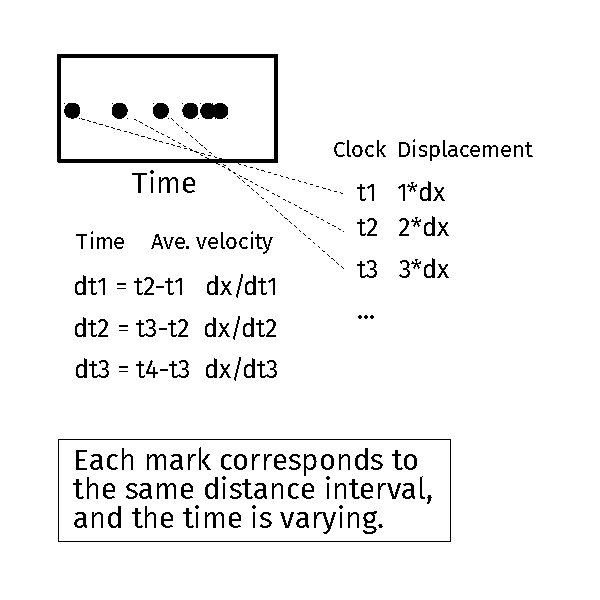
\includegraphics[width=0.55\textwidth]{figures/PicketG2.pdf}
\caption{\label{fig:picket2} We can measure the velocity versus time of the picket by taking the ratio of \textit{displacements} to \textit{times}.}
\end{figure}
\end{frame}

\begin{frame}{Lab Activity: Measuring acceleration of gravity}
\small
Acceleration is the change in velocity, so once we have the velocities ($dx/dt_{\rm i}$), we can take more ratios:
\begin{columns}[T]
\begin{column}{0.5\textwidth}
\begin{align}
t1' = (t2+t1)/2 & \quad dx/dt1 \\
t2' = (t3+t2)/2 & \quad dx/dt2 \\
t3' = (t4+t3)/2  & \quad dx/dt3 \\
...
\end{align}
\end{column}
\begin{column}{0.5\textwidth}
\begin{align}
t1' & \quad \frac{dx/dt2-dx/dt1}{t2'-t1'} \\
t2' & \quad \frac{dx/dt3-dx/dt2}{t3'-t2'}  \\
t3' & \quad \frac{dx/dt4-dx/dt3}{t4'-t3'}  \\
...
\end{align}
\end{column}
\end{columns}
\end{frame}

\begin{frame}{Lab Activity: Measuring acceleration of gravity}
Once we have the acclerations $\frac{dx/dt2-dx/dt1}{t2'-t1'}, ...$, we can compare them with each other and compute the \textit{average} and \textit{standard deviation}.\\
\begin{align}
\bar{a}_{\rm meas} &= N^{-1} \sum_{\rm i}^N a_{\rm meas,i} \\
\sigma^2_{\rm meas} &= N^{-1} \sum_{\rm i}^N (a_{\rm meas,i}-\bar{a}_{\rm meas})^2
\end{align} \\
Quote the result like this: $\bar{a}_{\rm meas}\pm\sigma_{\rm meas}$.  \textit{The mean plus or minus one standard deviation.}  The result of this experiment is $g = \bar{a}_{\rm meas}$, the acceleration due to gravity near the Earth's surface.
\end{frame}

\begin{frame}{Lab Activity: Measuring acceleration of gravity}
\small
\begin{figure}
\centering
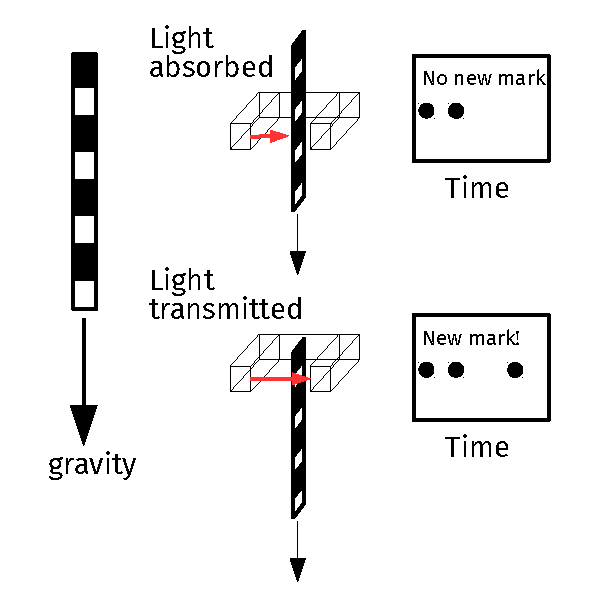
\includegraphics[width=0.5\textwidth]{figures/PicketG.pdf}
\caption{\label{fig:picket3} Does adding more mass to the picket change the answers?}
\end{figure}
\end{frame}

\section{Exercises with vectors, graphs, and equations of motion}

\begin{frame}{Exercises with vectors, graphs, and equations of motion}
We have a system of equations describing motion of classical particles undergoing constant acceleration:
\begin{align}
x &= x_{\rm 0} +\bar{v}t \\
\bar{v} &= (v+v_{\rm 0})/2 \\
v &= v_{\rm 0} + at \\
x &= x_{\rm 0} + v_{\rm 0} t + 	\frac{1}{2}at^2 \\
v^2 &= v_{\rm 0}^2 + 2a(x-x_{\rm 0})
\end{align}
\end{frame}

\begin{frame}{Exercises with vectors, graphs, and equations of motion}
A particle moves in a straight line with an initial velocity of 30 m/s and a constant acceleration of 30 m/s$^2$.  What is the displacement at $t=5$ seconds?  What is the velocity at $t=5$ seconds? \\
\begin{itemize}
\item A: 900 m, 180 m
\item B: 180 m, 525 m/s
\item C: 525 m, 180 m/s
\item D: 700 m, 200 m/s
\end{itemize}
\end{frame}

\begin{frame}{Exercises with vectors, graphs, and equations of motion}
A particle is moving at 5 m/s, 60 degrees with respect to the x-axis.  At $t=0$ seconds, it begins to accelerate at 1 m/s$^2$.  What is the speed after 3 seconds?\\
\begin{itemize}
\item A: 8 m/s
\item B: 4 m/s
\item C: -4 m/s
\item D: -8 m/s 
\end{itemize}
\end{frame}

\begin{frame}{Exercises with vectors, graphs, and equations of motion}
If the particle is at (0,0) at $t=0$, where is the particle at $t=3$ seconds? \\
\begin{itemize}
\item A: (7.5,13) m
\item B: (16.9,9.75) m
\item C: (9.75,16.9) m
\item D: (13,7.5) m 
\end{itemize}
\end{frame}

\begin{frame}{Exercises with vectors, graphs, and equations of motion}
\begin{columns}[T]
\begin{column}{0.4\textwidth}
\small
Which segment(s) of the motion described by the plot at right has $v\approx0$ (m/s)?
\begin{itemize}
\item A
\item B and D
\item C
\item E
\end{itemize}
\end{column}
\begin{column}{0.6\textwidth}
\begin{figure}
\centering
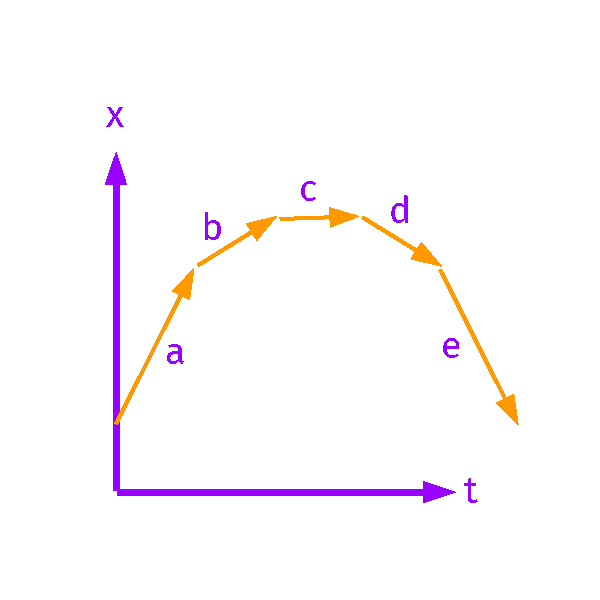
\includegraphics[width=\textwidth,trim=0cm 0cm 0cm 1.5cm,clip=true]{figures/Vectors2.pdf}
\end{figure}
\end{column}
\end{columns}
\end{frame}

\begin{frame}{Exercises with vectors, graphs, and equations of motion}
\begin{columns}[T]
\begin{column}{0.4\textwidth}
\small
Which segment(s) of the motion described by the plot at right has the largest velocity?
\begin{itemize}
\item A
\item B
\item D
\item E
\end{itemize}
\end{column}
\begin{column}{0.6\textwidth}
\begin{figure}
\centering
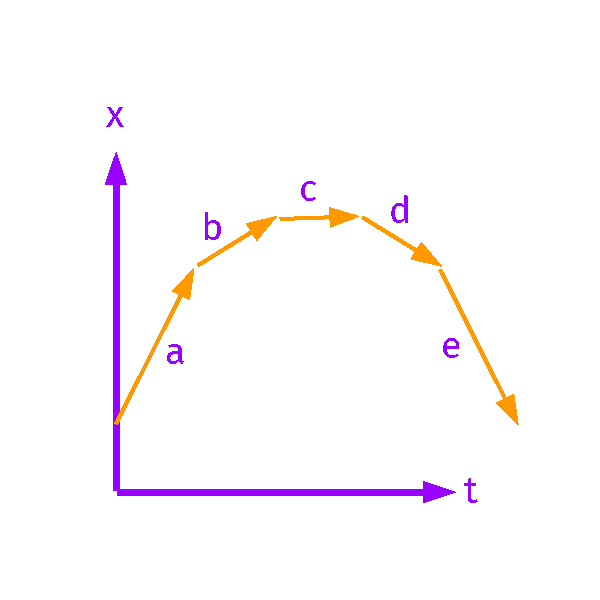
\includegraphics[width=\textwidth,trim=0cm 0cm 0cm 1.5cm,clip=true]{figures/Vectors2.pdf}
\end{figure}
\end{column}
\end{columns}
\end{frame}

\begin{frame}{Exercises with vectors, graphs, and equations of motion}
\begin{columns}[T]
\begin{column}{0.4\textwidth}
\small
Does the motion described by the plot correspond to negative or positive acceleration?
\begin{itemize}
\item Negative
\item Positive
\end{itemize}
\end{column}
\begin{column}{0.6\textwidth}
\begin{figure}
\centering
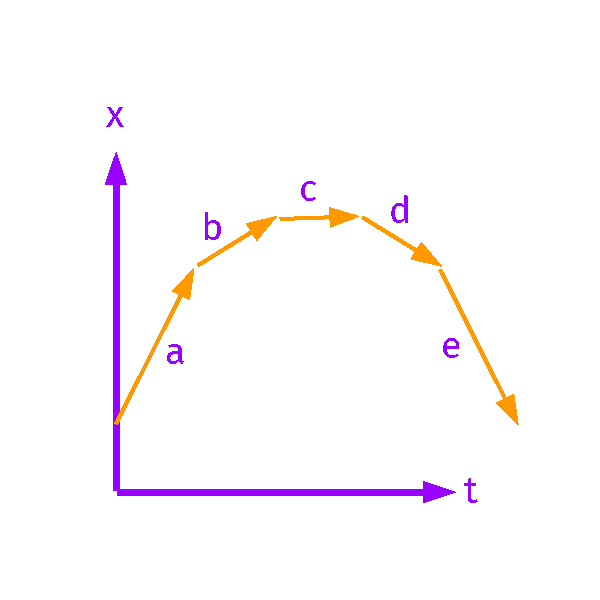
\includegraphics[width=\textwidth,trim=0cm 0cm 0cm 1.5cm,clip=true]{figures/Vectors2.pdf}
\end{figure}
\end{column}
\end{columns}
\end{frame}

\begin{frame}{Exercises with vectors, graphs, and equations of motion}
\begin{columns}[T]
\begin{column}{0.4\textwidth}
\small
In which region(s) is the acceleration zero m/s$^2$?
\begin{itemize}
\item A only
\item B only
\item Both A and B
\item None
\end{itemize}
\end{column}
\begin{column}{0.6\textwidth}
\begin{figure}
\centering
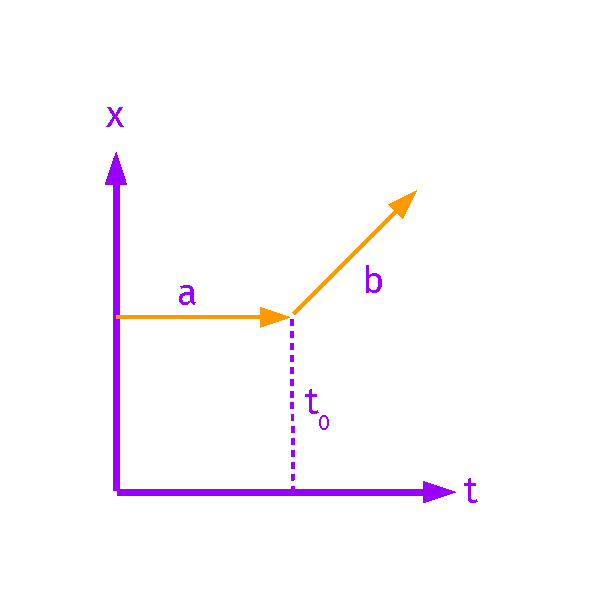
\includegraphics[width=\textwidth,trim=0cm 0cm 0cm 1.5cm,clip=true]{figures/Vectors3.pdf}
\end{figure}
\end{column}
\end{columns}
\end{frame}

\begin{frame}{Exercises with vectors, graphs, and equations of motion}
\begin{columns}[T]
\begin{column}{0.4\textwidth}
\small
At $t=t_{\rm 0}$, what is the acceleration?
\begin{itemize}
\item A: Negative and large
\item B: Positive and large
\item C: Positive, but small
\item D: Negative, but small
\end{itemize}
\end{column}
\begin{column}{0.6\textwidth}
\begin{figure}
\centering
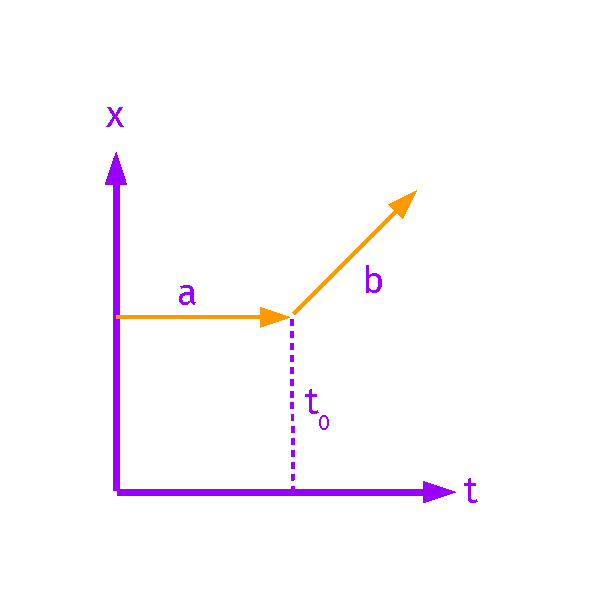
\includegraphics[width=\textwidth,trim=0cm 0cm 0cm 1.5cm,clip=true]{figures/Vectors3.pdf}
\end{figure}
\end{column}
\end{columns}
\end{frame}

\begin{frame}{Exercises with vectors, graphs, and equations of motion}
\begin{columns}[T]
\begin{column}{0.4\textwidth}
\small
What is the average velocity?
\begin{itemize}
\item A: Less than the slope of region B
\item B: Greater than the slope of region B
\item C: Zero
\item D: Similar to region B, but negative
\end{itemize}
\end{column}
\begin{column}{0.6\textwidth}
\begin{figure}
\centering
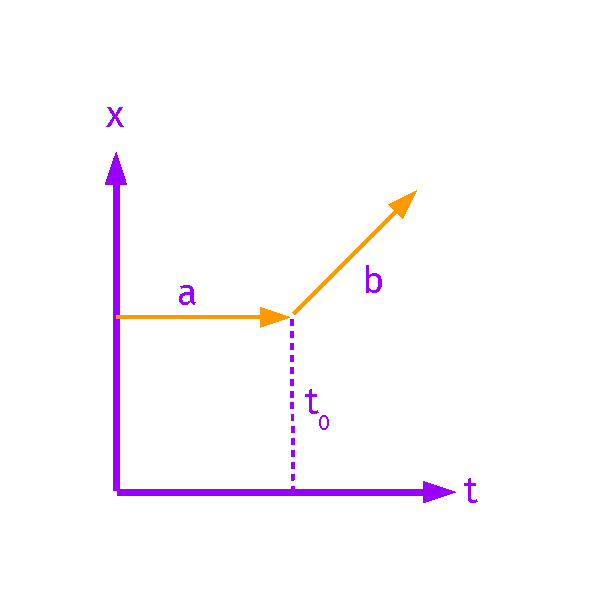
\includegraphics[width=\textwidth,trim=0cm 0cm 0cm 1.5cm,clip=true]{figures/Vectors3.pdf}
\end{figure}
\end{column}
\end{columns}
\end{frame}

\begin{frame}{Exercises with vectors, graphs, and equations of motion}
\begin{columns}[T]
\begin{column}{0.4\textwidth}
\small
What is the sign of the acceleration in region C?  What is the sign of the acceleration in going from region A to region B?
\begin{itemize}
\item Negative, positive
\item Positive, negative
\item Positive, positive
\item Negative, negative
\end{itemize}
\end{column}
\begin{column}{0.6\textwidth}
\begin{figure}
\centering
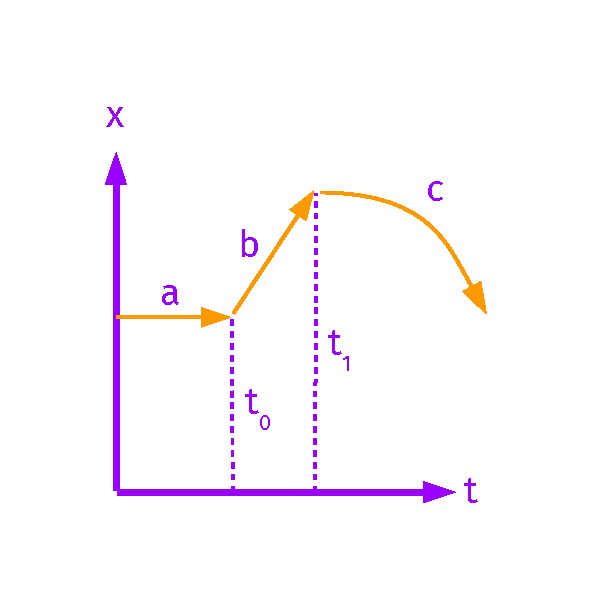
\includegraphics[width=\textwidth,trim=0cm 0cm 0cm 1.5cm,clip=true]{figures/FurtherExercises.pdf}
\end{figure}
\end{column}
\end{columns}
\end{frame}

\begin{frame}{Exercises with vectors, graphs, and equations of motion}
\begin{columns}[T]
\begin{column}{0.4\textwidth}
\small
What is most likely the total displacement?
\begin{itemize}
\item A: Positive and large
\item B: Negative and large
\item C: Zero
\item D: Cannot discern from graph
\end{itemize}
\end{column}
\begin{column}{0.6\textwidth}
\begin{figure}
\centering
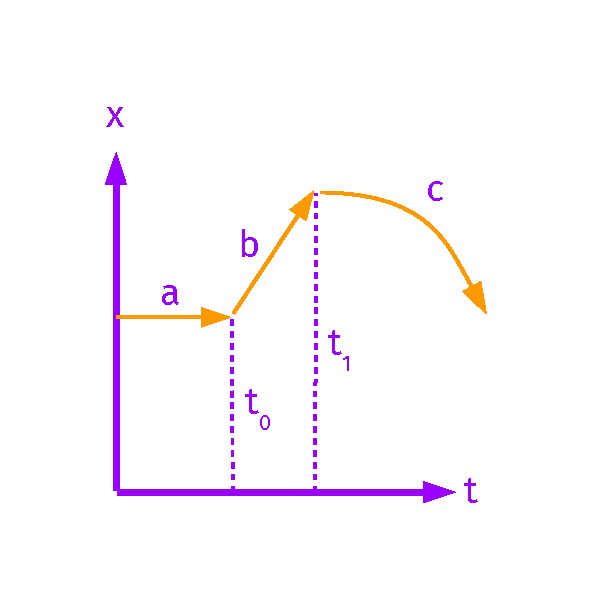
\includegraphics[width=\textwidth,trim=0cm 0cm 0cm 1.5cm,clip=true]{figures/FurtherExercises.pdf}
\end{figure}
\end{column}
\end{columns}
\end{frame}

\begin{frame}{Exercises with vectors, graphs, and equations of motion}
\begin{columns}[T]
\begin{column}{0.4\textwidth}
\small
What is most likely the acceleration during segment C?
\begin{itemize}
\item A: Positive and increasing
\item B: Negative and increasing
\item C: Negative and decreasing
\item D: Negative and constant
\end{itemize}
\end{column}
\begin{column}{0.6\textwidth}
\begin{figure}
\centering
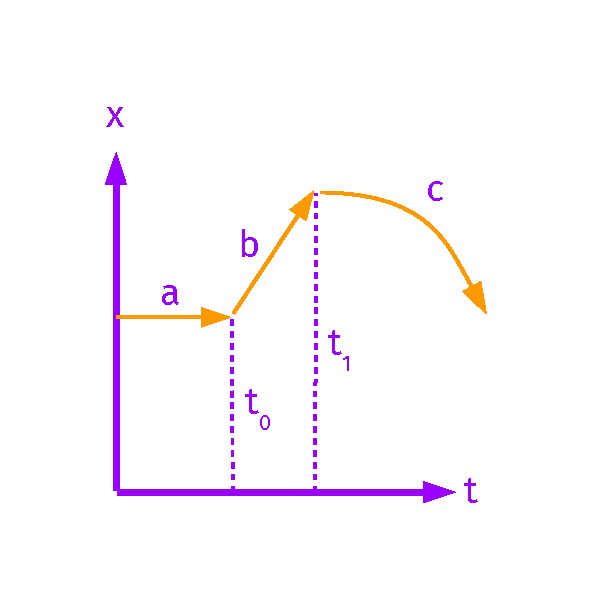
\includegraphics[width=\textwidth,trim=0cm 0cm 0cm 1.5cm,clip=true]{figures/FurtherExercises.pdf}
\end{figure}
\end{column}
\end{columns}
\end{frame}

\begin{frame}{Exercises with vectors, graphs, and equations of motion}
A particle is moving along the y-axis, with an initial speed of 10 m/s, and an acceleration of -10 m/s$^2$.  What is the displacement when the speed has decreased to 1 m/s?\\
\begin{itemize}
\item A: 3 m
\item B: 4 m
\item C: 5 m
\item D: 6 m
\end{itemize}
\end{frame}

\begin{frame}{Exercises with vectors, graphs, and equations of motion}
A particle is moving along the y-axis, with an initial speed of 10 m/s, and an acceleration of -10 m/s$^2$.  How much time has elapsed when the particle has a speed of 1 m/s?\\
\begin{itemize}
\item A: 0.9 seconds
\item B: 10 seconds
\item C: 0.5 seconds
\item D: 1.5 seconds
\end{itemize}
\end{frame}

\begin{frame}{Exercises with vectors, graphs, and equations of motion}
We have a gap in our abilities to solve problems with constant acceleration.  We can know how to use \textit{differentiation} to obtain other quantities/equations, including the approximate quantities of \textit{average velocity} and \textit{average acceleration}.  What about integration? \\
\begin{equation}
\int_{t_{\rm 1}}^{t_{\rm 2}} v(t) dt = x(t)
\label{eq:reverse1}
\end{equation}
Equation \ref{eq:reverse1} follows from the \textit{fundamental theorem of calculus} (more on this later).
\end{frame}

\begin{frame}{Exercises with vectors, graphs, and equations of motion}
A particle is moving along the z-axis, according to $\vec{v}(t) = (v_{\rm 0}-g_{\rm m}t) \hat{k}$ (m/s), where $v_{\rm 0} = 2$ (m/s) at $t=0$, and $g_{\rm m} = g/6$, the acceleration due to gravity on the moon (-9.8/6 m/s$^2$). What is the displacement after 2 seconds have elapsed?\\
\begin{itemize}
\item A: 4/3 m
\item B: 10/3 m
\item C: 1 m
\item D: 2/3 m
\end{itemize}
\end{frame}

\begin{frame}{Exercises with vectors, graphs, and equations of motion}
What about integration? \\
\begin{equation}
\int_{t_{\rm 1}}^{t_{\rm 2}} a(t) dt = v(t)
\label{eq:reverse2}
\end{equation}
Equation \ref{eq:reverse2} follows from the \textit{fundamental theorem of calculus} (more on this later).
\end{frame}

\begin{frame}{Exercises with vectors, graphs, and equations of motion}
At $t=0$, a particle has an acceleration $\vec{a}(t) = -(3\hat{i}+4\hat{j})$ m/s$^2$.  What is the velocity after 3 seconds?\\
\begin{itemize}
\item A: $(-3\hat{i}-4\hat{j})$ m/s
\item B: $(3\hat{i}+4\hat{j})$ m/s
\item C: $(-9\hat{i}-12\hat{j})$ m/s
\item D: $(-12\hat{i}-9\hat{j})$ m/s
\end{itemize}
\end{frame}

\section{Conclusion}

\begin{frame}{Week 2 Summary}
\begin{enumerate}
\item Displacement, and instantaneous velocity and acceleration
\begin{itemize}
\item \textit{Mathematics review}: taking derivatives
\item Average velocity and average acceleration
\end{itemize}
\item The case of constant acceleration
\begin{itemize}
\item An \textit{an equation of motion} for constant acceleration
\item Derivation of \alert{common equations of motion}
\item Average quantities and exercises
\end{itemize}
\item \textbf{Lab Activity: Measuring acceleration of gravity: \textit{g}}
\item Exercises with vectors, graphs, and equations of motion
\end{enumerate}
\end{frame}

\end{document}
